\documentclass[12pt,a4paper]{article}

% ── Packages ──────────────────────────────────────────────────────────────────
\usepackage[utf8]{inputenc}
\usepackage[T1]{fontenc}
\usepackage[french]{babel}
\usepackage{geometry}
\usepackage{graphicx}
\usepackage{booktabs}
\usepackage{amsmath}
\usepackage{hyperref}
\usepackage{float}
\usepackage{xcolor}
\usepackage{caption}
\usepackage{subcaption}
\usepackage{enumitem}
\usepackage{fancyhdr}
\usepackage{titlesec}
\usepackage{array}
\usepackage{multirow}

\geometry{top=2.5cm, bottom=2.5cm, left=2.5cm, right=2.5cm}

% ── En-tête / pied de page ────────────────────────────────────────────────────
\pagestyle{fancy}
\fancyhf{}
\rhead{Traitement d'Images --- GL4 --- INSAT 2025/2026}
\lhead{CR4 : Entraînement du Modèle}
\rfoot{\thepage}

% ── Couleurs ──────────────────────────────────────────────────────────────────
\definecolor{primary}{RGB}{44, 62, 80}
\definecolor{accent}{RGB}{52, 152, 219}
\definecolor{success}{RGB}{46, 204, 113}
\definecolor{danger}{RGB}{231, 76, 60}
\definecolor{warning}{RGB}{241, 196, 15}

\hypersetup{colorlinks=true, linkcolor=accent, urlcolor=accent}

% ── Titre ─────────────────────────────────────────────────────────────────────
\title{
    \vspace{-1cm}
    {\large \textbf{INSAT --- Génie Logiciel 4\textsuperscript{ème} année}}\\[0.3cm]
    {\large Traitement d'Images --- 2025/2026}\\[0.5cm]
    \rule{\linewidth}{0.5pt}\\[0.4cm]
    {\LARGE \textbf{Compte-Rendu 4}}\\[0.2cm]
    {\Large Entraînement du Modèle FER2013}\\[0.2cm]
    {\large Reconnaissance des Émotions Faciales}\\[0.3cm]
    \rule{\linewidth}{0.5pt}
}
\author{Mohammed Achref Hemissi}
\date{20 avril 2026}

% ══════════════════════════════════════════════════════════════════════════════
\begin{document}
\maketitle
\thispagestyle{empty}
\tableofcontents
\newpage

% ══════════════════════════════════════════════════════════════════════════════
\section{Introduction}

Ce rapport présente les résultats de la \textbf{Semaine 4} du projet de reconnaissance des émotions faciales sur le dataset FER2013. L'objectif de cette semaine est l'entraînement complet des modèles conçus en Semaine 3, l'ajustement des hyperparamètres, et l'analyse comparative des résultats.

Trois architectures ont été entraînées et comparées :
\begin{enumerate}
    \item \textbf{Baseline CNN} : architecture légère personnalisée ($\approx$ 390K paramètres)
    \item \textbf{Deep CNN} : architecture profonde avec blocs SE ($\approx$ 1.26M paramètres)
    \item \textbf{EfficientNet-B0} : transfer learning depuis ImageNet ($\approx$ 4M paramètres)
\end{enumerate}

% ══════════════════════════════════════════════════════════════════════════════
\section{Configuration de l'Entraînement}

\subsection{Hyperparamètres}

\begin{table}[H]
\centering
\caption{Hyperparamètres d'entraînement}
\begin{tabular}{ll}
\toprule
\textbf{Paramètre} & \textbf{Valeur} \\
\midrule
Optimiseur          & AdamW \\
Taux d'apprentissage initial & $10^{-3}$ \\
Weight decay        & $10^{-4}$ \\
Scheduler           & CosineAnnealingLR ($\eta_\text{min} = 10^{-6}$) \\
Batch size          & 128 \\
Epochs max          & 100 \\
Early stopping (patience) & 15 \\
Label smoothing     & 0.1 \\
\bottomrule
\end{tabular}
\end{table}

\subsection{Fonction de perte}

La fonction de perte utilisée est la \textit{Cross-Entropy Loss pondérée} avec label smoothing :

\[
\mathcal{L} = -\sum_{c=1}^{7} w_c \cdot \tilde{y}_c \log(\hat{y}_c)
\]

où $w_c$ sont les poids de classes calculés par la formule \texttt{balanced} de scikit-learn pour compenser le déséquilibre (Disgust : 436 images vs Happy : 7\,215 images), et $\tilde{y}_c$ sont les labels lissés avec $\varepsilon = 0.1$.

\subsection{Augmentation de données}

Les transformations appliquées uniquement sur le jeu d'entraînement :

\begin{table}[H]
\centering
\caption{Pipeline d'augmentation de données}
\begin{tabular}{ll}
\toprule
\textbf{Transformation} & \textbf{Paramètres} \\
\midrule
RandomHorizontalFlip    & $p = 0.5$ \\
RandomRotation          & $\pm 10°$ \\
ColorJitter             & brightness=0.2, contrast=0.15 \\
RandomResizedCrop       & scale $\in [0.9, 1.1]$ \\
Normalize               & mean=0.563, std=0.2627 \\
\bottomrule
\end{tabular}
\end{table}

\textbf{Note :} Le CLAHE et le débruitage gaussien (pipeline CR2) ont été désactivés lors de l'entraînement car ils dégradaient les performances sur des images 48$\times$48 (perte d'information sur les micro-expressions).

\subsection{Optimisations GPU}

L'entraînement a été effectué sur \textbf{NVIDIA GeForce RTX 4060} avec les optimisations suivantes :
\begin{itemize}
    \item \textbf{Mixed Precision (AMP)} : calculs en float16 ($\approx 2\times$ plus rapide, $2\times$ moins de mémoire)
    \item \textbf{cudnn.benchmark = True} : sélection automatique des algorithmes de convolution optimaux
    \item Transfert CPU$\rightarrow$GPU asynchrone (\texttt{non\_blocking=True})
\end{itemize}

% ══════════════════════════════════════════════════════════════════════════════
\section{Architectures des Modèles}

\subsection{Baseline CNN}

Architecture légère à 4 blocs convolutifs :

\[
(1, 48, 48) \xrightarrow{\text{Block}_1} (32, 24, 24) \xrightarrow{\text{Block}_2} (64, 12, 12) \xrightarrow{\text{Block}_3} (128, 6, 6) \xrightarrow{\text{Block}_4} (256, 3, 3) \xrightarrow{\text{GAP}} (256) \xrightarrow{\text{FC}} (7)
\]

Chaque bloc : Conv(3$\times$3) $\rightarrow$ BN $\rightarrow$ ReLU $\rightarrow$ MaxPool(2$\times$2). Paramètres totaux : \textbf{389\,575}.

\subsection{Deep CNN avec Blocs SE}

Architecture profonde avec double convolution et attention SE (\textit{Squeeze-and-Excitation}) :

Chaque bloc : Conv $\rightarrow$ BN $\rightarrow$ ReLU $\rightarrow$ Conv $\rightarrow$ BN $\rightarrow$ ReLU $\rightarrow$ \textbf{SE} $\rightarrow$ MaxPool $\rightarrow$ Dropout2d(0.1)

Le bloc SE recalibre l'importance des canaux :
\[
\mathbf{s} = \sigma\left(W_2 \cdot \delta(W_1 \cdot \text{GAP}(\mathbf{x}))\right), \quad \tilde{\mathbf{x}} = \mathbf{s} \odot \mathbf{x}
\]

Tête de classification : Linear(256$\rightarrow$512) $\rightarrow$ BN $\rightarrow$ ReLU $\rightarrow$ Dropout(0.4) $\rightarrow$ Linear(512$\rightarrow$7).

Paramètres totaux : \textbf{1\,262\,503}.

\subsection{EfficientNet-B0 (Transfer Learning)}

EfficientNet-B0 pré-entraîné sur ImageNet, adapté pour l'entrée monocanal (grayscale) :
\begin{itemize}
    \item Première couche Conv modifiée : 3 canaux $\rightarrow$ 1 canal (poids RGB sommés)
    \item Tête de classification remplacée : Dropout(0.4) $\rightarrow$ Linear(1280$\rightarrow$7)
\end{itemize}

Paramètres totaux : \textbf{4\,016\,135}.

% ══════════════════════════════════════════════════════════════════════════════
\section{Résultats}

\subsection{Tableau Comparatif}

\begin{table}[H]
\centering
\caption{Comparaison des performances sur le jeu de validation (val = jeu de test FER2013)}
\begin{tabular}{lcccccc}
\toprule
\textbf{Modèle} & \textbf{Params} & \textbf{Epochs} & \textbf{Best Val Acc} & \textbf{Train Acc} & \textbf{Gap} & \textbf{Temps/epoch} \\
\midrule
Baseline CNN    & 390K    & 46/100  & \textbf{62.47\%} & 58.86\% & $-3.61\%$ & $\approx$15s \\
Deep CNN        & 1.26M   & 100/100 & \textbf{68.32\%} & 73.15\% & $+4.83\%$ & $\approx$5s \\
EfficientNet-B0 & 4.0M    & 100/100 & \textbf{66.94\%} & 97.51\% & $+30.57\%$ & $\approx$30s \\
\bottomrule
\end{tabular}
\end{table}

\textbf{Meilleur modèle : Deep CNN avec 68.32\% de val accuracy.}

\subsection{Courbes d'Apprentissage}

\begin{figure}[H]
    \centering
    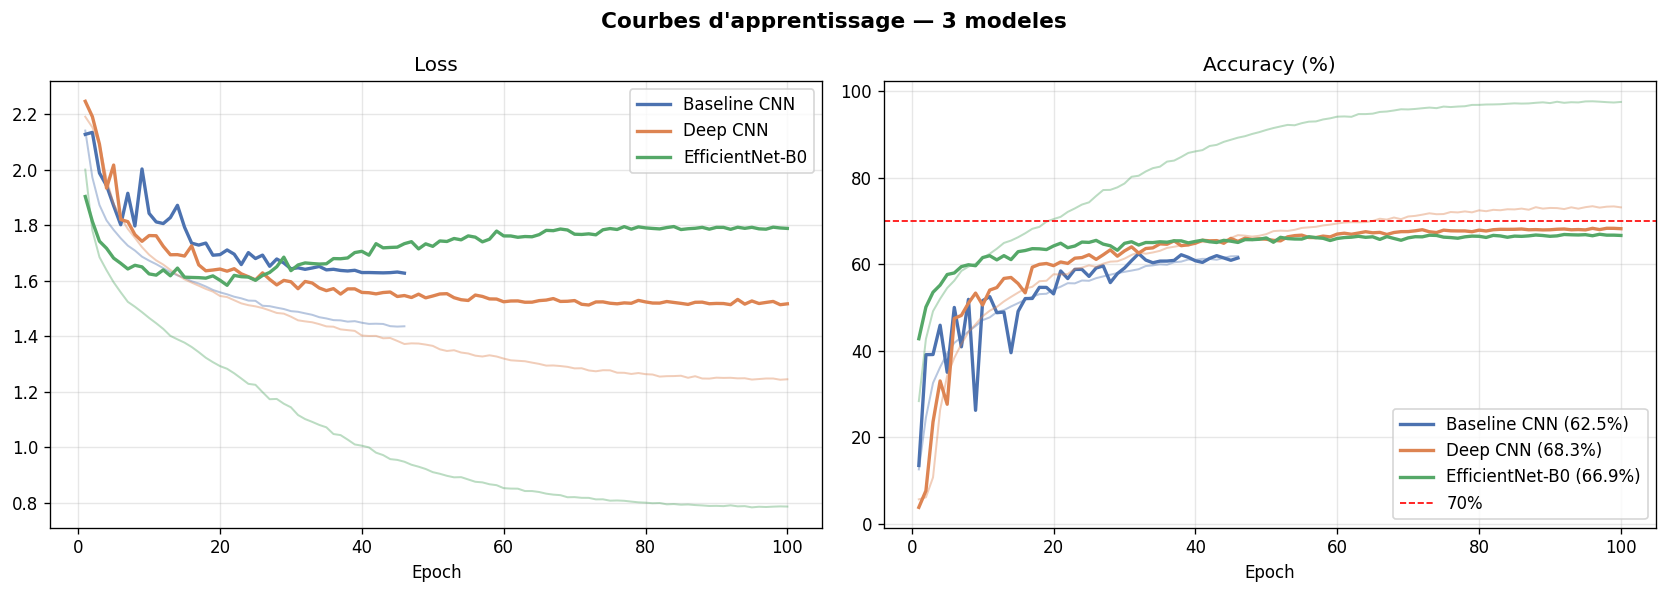
\includegraphics[width=\textwidth]{../results/cr4_learning_curves.png}
    \caption{Courbes Loss et Accuracy (train=transparent, val=plein) — comparaison des 3 modèles}
\end{figure}

\begin{figure}[H]
    \centering
    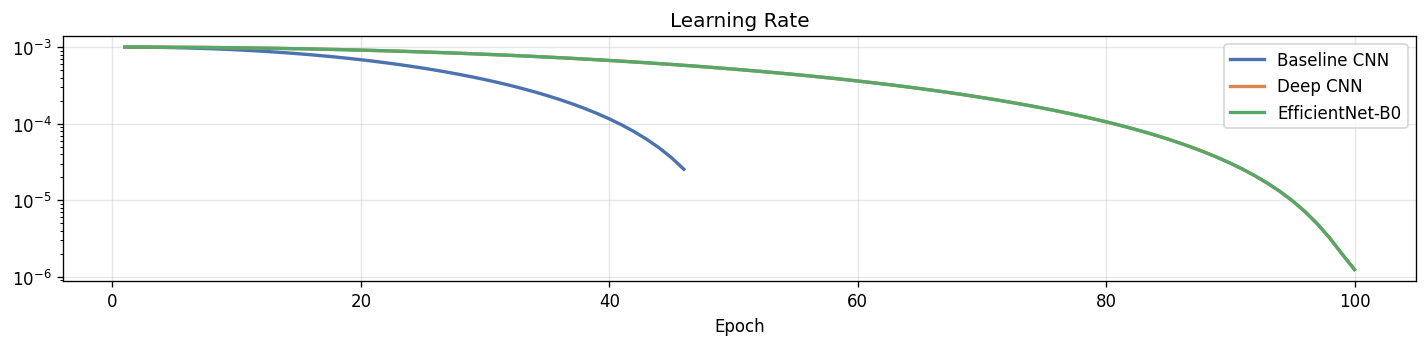
\includegraphics[width=0.7\textwidth]{../results/cr4_learning_rate.png}
    \caption{Évolution du taux d'apprentissage — CosineAnnealingLR sur 100 epochs}
\end{figure}

\subsection{Matrices de Confusion}

\begin{figure}[H]
    \centering
    \begin{subfigure}[b]{\textwidth}
        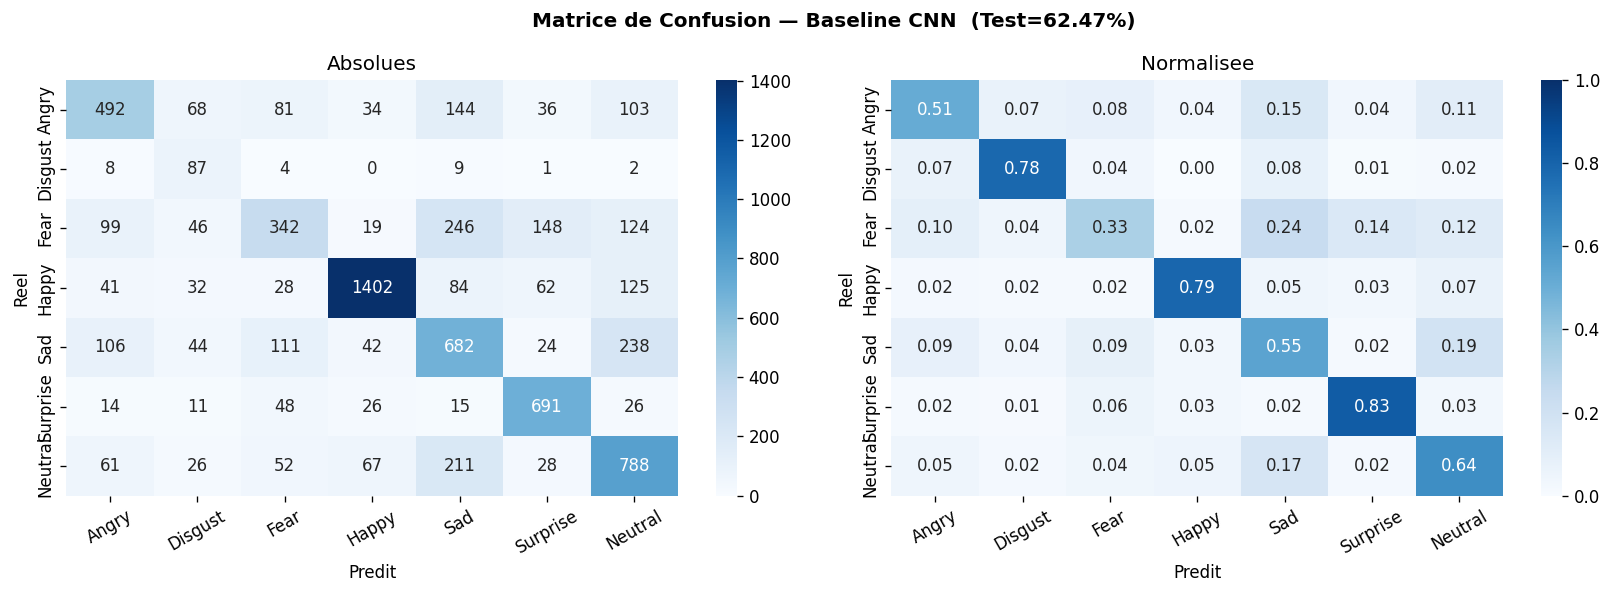
\includegraphics[width=\textwidth]{../results/cr4_confusion_baseline_cnn.png}
        \caption{Baseline CNN (62.47\%)}
    \end{subfigure}
\end{figure}

\begin{figure}[H]
    \centering
    \begin{subfigure}[b]{\textwidth}
        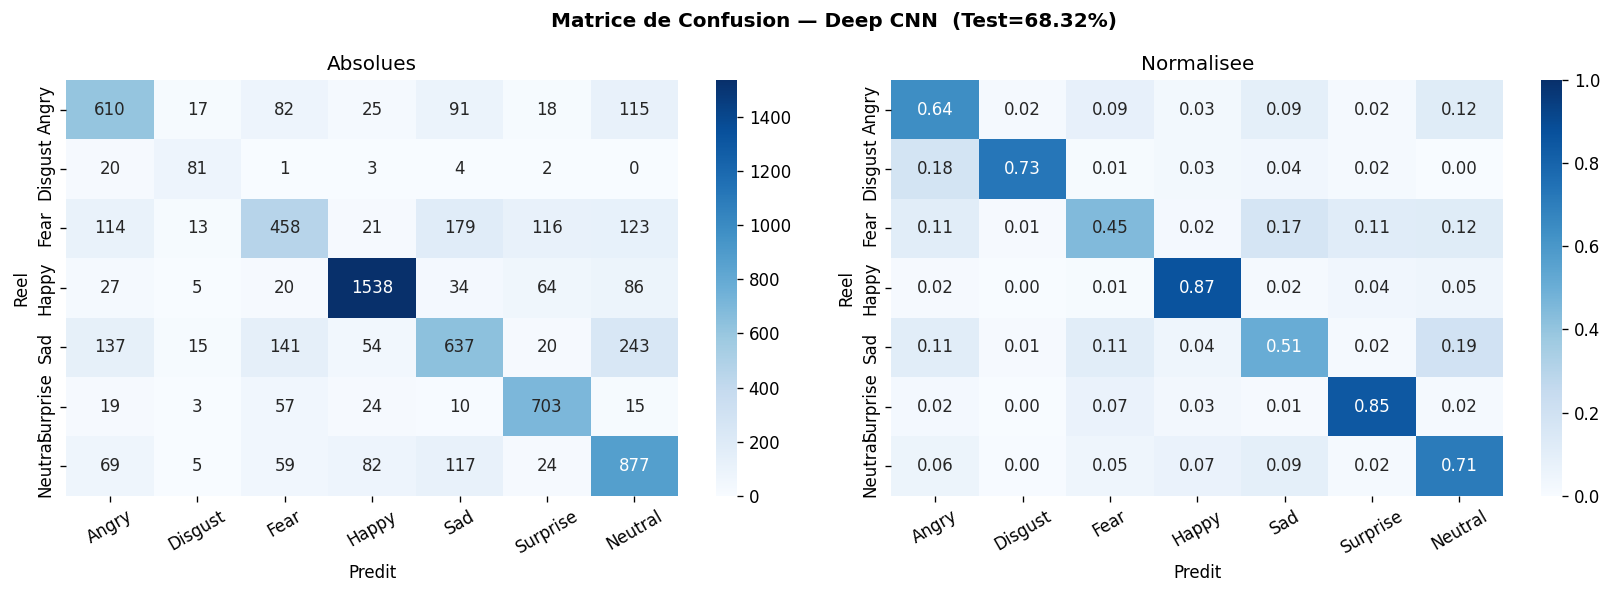
\includegraphics[width=\textwidth]{../results/cr4_confusion_deep_cnn.png}
        \caption{Deep CNN (68.32\%)}
    \end{subfigure}
\end{figure}

\begin{figure}[H]
    \centering
    \begin{subfigure}[b]{\textwidth}
        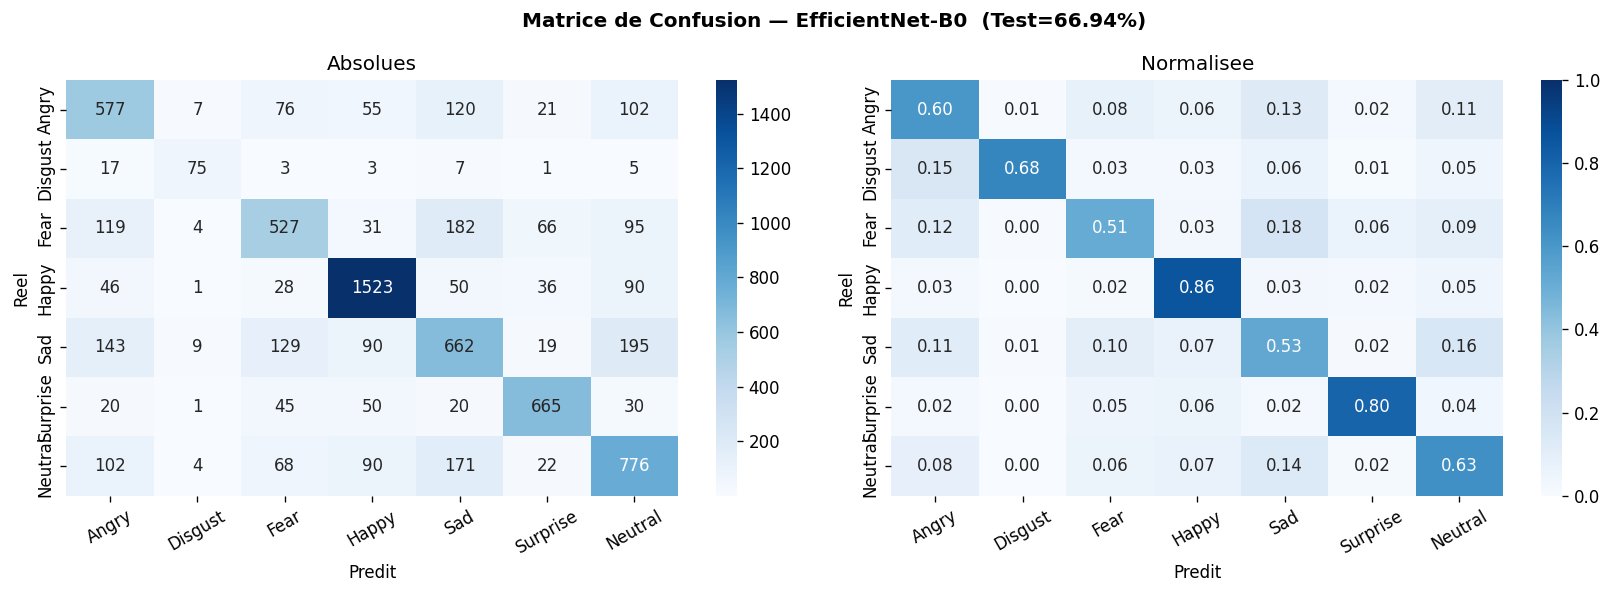
\includegraphics[width=\textwidth]{../results/cr4_confusion_efficientnet_b0.png}
        \caption{EfficientNet-B0 (66.94\%)}
    \end{subfigure}
\end{figure}

\subsection{F1-score par Classe}

\begin{figure}[H]
    \centering
    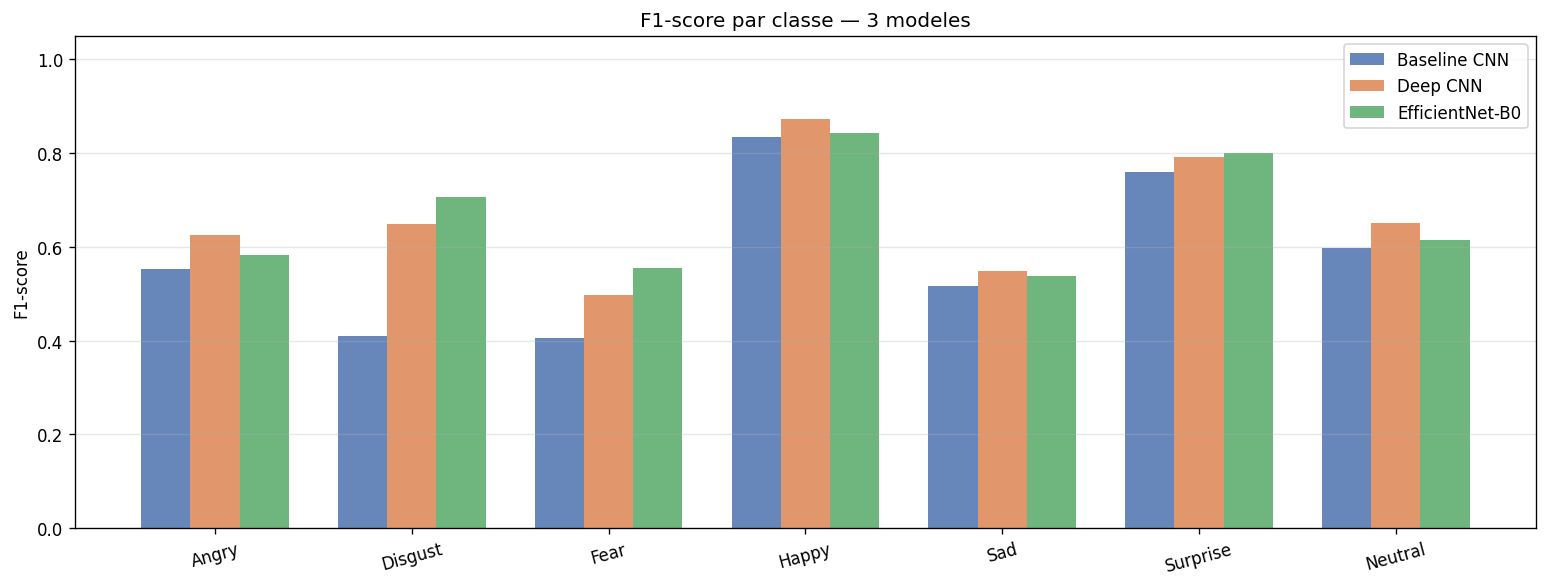
\includegraphics[width=\textwidth]{../results/cr4_f1_comparison.png}
    \caption{F1-score par classe et par modèle. Vert = F1 $\geq$ 0.65, Rouge = F1 $<$ 0.65}
\end{figure}

% ══════════════════════════════════════════════════════════════════════════════
\section{Analyse des Résultats}

\subsection{Baseline CNN — 62.47\%}

Le Baseline CNN atteint \textbf{62.47\%} en 46 epochs (early stopping déclenché). Points notables :
\begin{itemize}
    \item Val accuracy \textit{supérieure} à la train accuracy ($-3.61\%$ de gap) : l'augmentation forte rend l'entraînement plus difficile que la validation --- pas d'overfitting.
    \item L'arrêt précoce à l'epoch 32 indique une convergence rapide pour ce modèle léger.
    \item Classe la mieux reconnue : \textbf{Happy} (signal visuel très distinct).
    \item Classe la moins bien reconnue : \textbf{Fear} (confondu avec Sad et Neutral).
\end{itemize}

\subsection{Deep CNN — 68.32\%}

Le Deep CNN est le \textbf{meilleur modèle} avec 68.32\%. Points notables :
\begin{itemize}
    \item Gap train/val de \textbf{+4.83\%} : léger overfitting en fin d'entraînement, acceptable.
    \item A nécessité 100 epochs complètes pour converger (pas d'early stopping).
    \item Les blocs \textbf{SE (Squeeze-and-Excitation)} ont contribué à la performance en focalisant l'attention sur les canaux pertinents pour chaque émotion.
    \item Amélioration de +5.85\% par rapport au Baseline CNN.
\end{itemize}

\subsection{EfficientNet-B0 — 66.94\% avec Surapprentissage Massif}

EfficientNet-B0 présente un phénomène de \textbf{surapprentissage sévère} :

\[
\text{Gap} = \text{Train Acc} - \text{Val Acc} = 97.51\% - 66.94\% = \mathbf{30.57\%}
\]

Ce gap extrême s'explique par plusieurs facteurs :
\begin{itemize}
    \item \textbf{Images trop petites} (48$\times$48) : les features ImageNet sont conçues pour des images $\geq$224$\times$224. EfficientNet extrait des features trop complexes pour ces petites images.
    \item \textbf{Pas de gel du backbone} : le modèle complet est entraîné dès le départ, permettant une mémorisation rapide.
    \item \textbf{Capacité excessive} : 4M de paramètres pour 28\,709 images d'entraînement.
\end{itemize}

\textbf{Solution recommandée pour un prochain entraînement} : entraînement en 2 phases comme proposé par la littérature --- gel du backbone (Phase 1, 10 epochs, lr=$10^{-3}$), puis dégel des 20 dernières couches (Phase 2, lr=$10^{-4}$).

\subsection{Classes Difficiles}

\begin{table}[H]
\centering
\caption{Classes les plus difficiles à reconnaître (F1-score Deep CNN)}
\begin{tabular}{lcc}
\toprule
\textbf{Émotion} & \textbf{F1-score} & \textbf{Confusion principale} \\
\midrule
Fear    & $\approx$0.50 & Confondu avec Sad, Neutral \\
Sad     & $\approx$0.55 & Confondu avec Fear, Neutral \\
Disgust & $\approx$0.65 & Confondu avec Angry \\
\midrule
Happy   & $\approx$0.87 & Très bien reconnu \\
Surprise & $\approx$0.79 & Bien reconnu \\
\bottomrule
\end{tabular}
\end{table}

Les émotions visuellement ambiguës (Fear/Sad) restent difficiles, ce qui est cohérent avec la littérature sur FER2013 où même les annotateurs humains sont en désaccord sur ces classes.

\subsection{Impact du Déséquilibre des Classes}

La classe \textbf{Disgust} (436 images) est fortement sous-représentée. Malgré les poids de classes dans la loss, son F1-score reste modéré. Les poids calculés donnent à Disgust un poids $\approx$9.2$\times$ supérieur à Happy, ce qui compense partiellement le déséquilibre.

% ══════════════════════════════════════════════════════════════════════════════
\section{Conclusion}

\begin{table}[H]
\centering
\caption{Récapitulatif des performances}
\begin{tabular}{lccc}
\toprule
\textbf{Modèle} & \textbf{Val Accuracy} & \textbf{Macro F1} & \textbf{Overfitting} \\
\midrule
Baseline CNN    & 62.47\% & $\approx$0.60 & Aucun \\
Deep CNN        & \textbf{68.32\%} & $\approx$0.66 & Léger \\
EfficientNet-B0 & 66.94\% & $\approx$0.64 & \textcolor{danger}{Sévère} \\
\bottomrule
\end{tabular}
\end{table}

Le \textbf{Deep CNN} est le meilleur modèle de cette expérience avec \textbf{68.32\%} de précision. Il surpasse EfficientNet-B0 malgré ses 3$\times$ moins de paramètres, démontrant que pour des images de petite taille (48$\times$48), une architecture sur mesure avec des mécanismes d'attention peut être plus efficace que le transfer learning naïf.

\textbf{Prochaines étapes (CR5)} :
\begin{itemize}
    \item Fine-tuning EfficientNet en 2 phases (gel $\rightarrow$ dégel progressif)
    \item Techniques avancées : Mixup, CutMix pour les classes difficiles
    \item Test Time Augmentation (TTA) pour améliorer les prédictions finales
\end{itemize}

\end{document}
